\documentclass{article}
\usepackage[UTF8]{ctex}
\usepackage{geometry}
\usepackage{float}
\usepackage{natbib}
\geometry{left=3.18cm,right=3.18cm,top=2.54cm,bottom=2.54cm}
\usepackage{graphicx}
\pagestyle{plain}	
\usepackage{setspace}
\usepackage{caption2}
\usepackage{datetime} %日期
\renewcommand{\today}{\number\year 年 \number\month 月 \number\day 日}
\renewcommand{\captionlabelfont}{\small}
\renewcommand{\captionfont}{\small}
\begin{document}

\begin{figure}
    \centering
    
\includegraphics[width=8cm]{upc.png}

    \label{figupc}
\end{figure}

	\begin{center}
		\quad \\
		\quad \\
		\heiti \fontsize{45}{17} \quad \quad \quad 
		\vskip 1.5cm
		\heiti \zihao{2} 《计算科学导论》课程总结报告
	\end{center}
	\vskip 2.0cm
		
	\begin{quotation}
% 	\begin{center}
		\doublespacing
		
        \zihao{4}\par\setlength\parindent{7em}
		\quad 

		学生姓名:\underline{\qquad  李伟峰 \qquad \qquad}

		学\hspace{0.61cm} 号:\underline{\qquad 2007010213\qquad}
		
		专业班级:\underline{\qquad 计科2002 \qquad  }
		
        学\hspace{0.61cm} 院:\underline{计算机科学与技术学院}
% 	\end{center}
		\vskip 2cm
		\centering
		\begin{table}[h]
            \centering 
            \zihao{4}
            \begin{tabular}{|c|c|c|c|c|c|c|}
            % 这里的rl 与表格对应可以看到,姓名是r,右对齐的;学号是l,左对齐的;若想居中,使用c关键字。
                \hline
                课程认识 & 问题思 考 & 格式规范  & IT工具  & Latex附加  & 总分 & 评阅教师 \\
                30\% & 30\% & 20\% & 20\% & 10\% &  &  \\
                \hline
                 & & & & & &\\
                & & & & & &\\
                \hline
            \end{tabular}
        \end{table}
		\vskip 2cm
		\today
	\end{quotation}

\thispagestyle{empty}
\newpage
\setcounter{page}{1}

\section{引言}
	随着计算机科学技术的不断发展,21世纪已成为了信息爆炸的时代,信息量呈几何倍数增长。计算机已成为了我们生活中的一部分。
现今社会中的方方面面越来越依赖于计算机的应用。正因如此,它对人类发展有着密不可分的关系。计算科学作为一门基础学科,介绍了计算机各个领域的内容。
计算机导论系统而全面的描述了计算科学的发展及其结构组成。经过这一学期的学习,我对计算科学也有了一些自己的认识与思考。

\section{对计算科学导论这门课程的认识、体会}
“计算科学导论”,顾名思义,是一个对计算机专业的概括性、引导性的课程。导论也称作引论,
是论著正文前概要论述全文或全书的中心思想、创作思路、背景和创作方向的简单概括叙述,以指导帮助读者阅读理解的部分。
关于学科的导论是指用较为概括的语言来论述这一学科的基本的和整体的思想,从而使读者对该学科有较为整体和系统的把握。\par
在上这门课之前,我觉得自己对计算机专业还是有大致的了解的,因为自身的兴趣,我接触这方面的时间比较早,在高中也参加过相关的竞赛,主要对算法方面有一定的了解,但是对计算机科学这门学科整体缺乏一个系统的了解。
直到学习了“计算科学导论”后,我才意识到计算机专业不止有“计算机科学与技术”,还有更深层次的“哲学”需要我们去探索。这已经不是技术层面的理解了,是从思想层面的层层深入。\par
\subsection{课程目录与主要内容}
\begin{itemize}
	\item 第一章:引论。本章主要讲计算科学一词的来历和计算科学的研究方法,旨在为读者提供研读本书的正确方法。
	\item 第二章:计算科学的基本概念和基本知识。本章介绍了计算模型与二进制,通用数字计算机系统结构与工作原理,数字逻辑与集成电路,机器指令与汇编语言,算法、过程与程序,高级语言与程序设计,系统软件与应用软件,计算机组织与体系结构,并行计算机、通道与并行计算,计算机网络与通信,计算机图形学与图像处理,逻辑与人工智能到数据处理与演化计,计算机科学与技术一级学科等领域内的一些重要的基本概念。
	\item 第三章:计算科学:它的意义、内容和方法。本章围绕计算机科学与技术学科的定义、特点、基本问题、发展主线、主流方向、学科方法论、历史渊源、发展变化、知识组织结构与分类体系、学科发展的潮流与未来发展方向以及组织结构及其演变。
	\item 第四章:如何学习计算机科学和健康成长。本章就学科人才培养目标、教学重点与科学素养等内容进行了系统而又深入浅出的论述,以科学办学思想和内涵发展优先的理念为基础,全面阐述了在培养计算机科学与技术一级学科创新人才与高素质专业技术开发人才的过程中,如何使学生正确地认识和学好计算机科学与技术学科。
	\item 第五章:布尔代数基础。本章介绍了一些主要的算法以及计算科学的应用。
	\end{itemize}
\subsection{科学哲学的思想方法}
本章的开头提到了一句话——真正理解一件事物最好的方式莫过于去探寻它的历史。
当一件事物、一个学科发展几年、几十年甚至几百年时,大多数人对这个已经略显成熟的甚至已经止于至善的事物的认识可能只有它所有最新的理论,最通俗的认知。
但是如果想深入地认识这个事物,单纯的从艰深的理论,最新的成果去深入研究是效率低下的。最好的方法其实是追本溯源,追溯到这个理论的源头,认识到它是为什么被提出来的,又是作为什么被研究的。
理解了根源之后,沿着该事物的发展路线,逐步学习、消化它所积淀的知识,才能完全的掌握理论,为己所用。\par
“计算科学”一词的来历可以追溯到20世纪30年代到60年代初,当时的工作主要是围绕“什么是计算”开展理论探索,数学问题主要还是靠科学家、数学家手工进行运算。直到图灵机的出现,才有了自动装置计算的开始,
后来有冯•诺依曼等人的贡献,1946年制造出了世界第一台大型计算机“ENAIC”。有了计算机强劲算力的支撑与高级程序设计语言的发展,计算数学的发展突飞猛进,同时多个领域的融合分化催生了计算机科学作为一个学科的出现。
经过发展,计算机科学又分化出了计算机科学与计算机工程两大阵营,各有侧重点,通俗来讲即一个偏研究,一个偏应用。分化的两大阵营也引起了很多争议与辩论,为了解决分歧,探索一个科学的发展方向,选择了“计算作为一门学科”
这个方向,计算学科囊括了计算机工程、信息技术、信息系统等18个主领域。所以“计算科学导论”其实是“计算机科学导论”的一个超集,概括性更强,有更深厚的历史积淀。\par
科学哲学 \citep{curd1998philosophy} 是20世纪兴起的一个哲学分支,关注科学的基础、方法和含义,主要研究科学的本性、科学理论的结构、科学解释、科学检验、科学观察与理论的关系、科学理论的选择等。该学科的中心问题是:
什么有资格作为科学,科学理论的可靠性,和科学的终极目的。此学科有时与形而上学、本体论和认识论重叠,例如当它探索科学与真理之间的关系时。\par
有许多关于科学哲学的核心问题,包括科学能否揭示不可观察之事物的真相,甚至科学推理是否可以被证明为合理的,哲学家们没有达成共识。除了这些关于科学作为一个整体的一般性问题,
科学哲学家也思考适用于特定学科例如生物学和物理学的问题。一些科学哲学家还使用当代的科学结果来达到哲学本身的结论。\par
但是我们要意识到:我们应该相信科学,迄今为止科学方法是我们能够发现具有真理性知识的最高方法,但是我们也不能迷信科学、迷信科学家,我们要有自己的判断力。
在面对科学结论时,我们需要自己审视它本身的科学性问题,这就是对我们的科学素养、科学常识的考验了。

\subsection{计算科学的意义、内容和方法}
什么是计算科学?计算科学是对描述和变换信息的算法过程,包括其理论、分析、设计、效率分析、实现和应用的系统研究。与第一章一样,这里主要要区分的就是“计算科学”与“计算机科学”,虽然只差了一个字,但是所代表的意义大有不同。\par
计算科学的问题域包括数值模拟、模型拟合与数据分析计算优化等领域。同时计算科学中的算法和数学方法也是多样的,
计算科学应用程序常常建立真实世界变化情况的模型,包括天气、飞机周围的气流、事故中的汽车车身变形、星系中恒星的运动、爆炸装置等。这类程序会在计算机内存中建立一个“逻辑网格”,网格中的每一项在空间上都对应一个区域,
并包含与模型相关的那一空间的信息。例如在天气模型中,每一项都可以是一平方千米,并包含了地面海拔、当前风向、温度、压力等。程序会在模拟时步中基于当前状态计算出可能的下一状态,解出描述系统运转方式的方程,然後重复上述过程计算出下一状态。
“计算科学家”一词常用于描述科学计算领域中的技能高超者。他们通常是科学家、统计学家或应用数学家,会以不同方式应用高性能计算机,以提高他们各自的应用学科(如物理学、化学或工程学的相关学科)中最先进的理论和技术水平。科学计算也对经济学、生物学及医学等领域有着越来越大的影响。
计算科学常被认为是科学的第三种方法,是实验/观察和理论这两种方法的补充和扩展。计算科学的本质是数值算法以及计算数学。在发展科学计算算法、程序设计语言的有效实现以及计算结果确认上,人们已经做出了实质性的努力。计算科学中的一系列问题和解决方法都可以在相关文献中找到。\citep{zxx}\par
计算科学自出现至今已经迭代多次,推动计算科学发展的主要动力便是社会广泛的应用需求。从目前来看,计算模型与体系结构、软件开发方法学与计算机应用技术是本学科未来发展的主要方向,而计算理论、体系结构、高等逻辑与形式语义学是支撑学科未来主要方向发展的四大核心专业知识基础。\par
计算科学的意义并没有在内容中出现,我自己进行了总结:计算科学为人类认知世界提供了一种可能的有前途的方法,自出现至今已经引起了人类世界观自然观的巨大变革。而计算机科学和信息科学的极大成就促进了计算概念的普遍化,计算科学为意识提供了一种主流的解释方法,为人工智能技术的发展提供了理论支撑,为理解生命以及基因技术的发展和基于生命科学的计算机技术等提供了理论纲领,有非凡的意义。

\section{进一步的思考}
我与我的搭档所演讲的内容是“密码学”,通过后续查阅相关文献,对于演讲中未能提及的问题做一个补充。\par
\subsection{密码学概述}
\subsubsection{密码学发展史}
密码学是一门非常古老的学科,早期的密码技术是把人们能够读懂的消息变换成不易读懂的信息用来隐藏信息内容,使得窃听者无法理解消息的内容,同时又能够让合法用户把变换的结果还原成能够读懂的消息。密码学的发展大致可以分为4个阶段。\citep{zhaodong}
即:\par
\begin{itemize}
    \item 手工阶段:代表有古罗马Caeser密码,法国Vigenere密码等。
    \item 机械阶段:代表是二战时期德国的恩尼格码密码机。
    \item 近现代阶段:随着通信、电子和计算机等技术的发展, 密码学得到前所未有的系统发展。1949年, Shannon发表了“保密系统的通信理论, 给出了密码学的数学基础, 证明了一次一密密码系统的完善保密性,基于香农的一系列论文,密码学正式被推上了基于信息论的科学轨道,后来产生了数据加密标准” (DES)算法 ,这其中的很多思想,奠定了现代密码设计的基石
    \item 现代阶段:在1976年, Diffie和Hellman提出了“密码学新方向”, 开辟了公钥密码技术理论, 使得密钥协商、数字签名等密码问题有了新的解决方法, 也为密码学的广泛应用奠定了基础。
\end{itemize}
\subsubsection{密码学基本概念与分类}
\begin{itemize}
    \item 密码编码学:把来自信息源的可理解的原始消息变换成不可理解的消息, 同时又可恢复到原消息的方法和原理的一门科学。
    \item 密码分析学:在不知道关于密钥的任何信息这一情况下, 利用各种技术手段, 试图通过密文来得到明文或密钥的全部信息或部分信息。密码分析也称为对密码体制的攻击。
\end{itemize}
\subsubsection{密码学发展趋势}
\begin{itemize}
    \item 标准化趋势:密码的标准化是密码理论与技术不断发展的结晶和原动力, 包括AES、安全哈希算法 (Secure Hash Algorithm 3, SHA3) 、以及eSTREAM计划和NESSE计划等都极大地推动了密码的标准化是密码理论与技术不断发展的结晶和原动力, 包括AES、安全哈希算法 (Secure Hash Algorithm 3, SHA3) 、以及eSTREAM计划和NESSE计划等都极大地推动了密码学研究。
    \item 公理化趋势:在设计密码算法的过程中, 保证算法的可证明安全性是非常有吸引力的, 密码协议的形式化分析方法、安全多方计算理论、可证明安全性理论以及零知识证明等仍将是密码协议研究中的主流方向。
    \item 面向社会的实用化趋势:随着电子政务和电子商务的出现, 密码技术的实际应用面临着新的机遇和挑战。基于生物特征的密码技术是目前研究的一个热点, 由于实际应用的需要, 它也是未来的一个重要研究方向。此外, 轻量级密码技术也已成为当前非常受关注的一个研究方向。
\end{itemize}
\subsection{量子时代的密码学}
量子计算模型所带来的巨大算力对于现有的密码体制有着巨大的威胁,我们需要探索新的密码体制以应对。
\subsubsection{现阶段量子计算技术对于目前密码体系的影响}
通用量子计算机器件进展缓慢,对实用化1024bit的RSA密码破译尚不能构成威胁,现代密码依旧是安全的. 量子计算密码攻击需要探索新的途径\citep{wangchao}
\subsubsection{后量子密码技术}
在量子计算模型下, 基于大整数分解和基于离散对数问题的密码体制将不再安全,同时所有基于攻击者计算复杂性假设而构造的密码算法(无论是对称还是非对称算法)的安全性也非常值得怀疑。 人们需要找到能够代替这类经典算法的密码体制, 希望能够抵抗量子计算攻击。
对于后量子密码(PQC)算法,我们着重指那些在大规模量子计算机出现后仍保持计算安全的密码算法。这些算法的构造没有采用量子力学的物理特性,而是延续传统主流的计算上的可证安全研究方法。
目前,后量子算法的研究重点是构造解决公钥加密(密钥建立)和签名问题的非对称算法,主要包括基于格、编码、多变量多项式以及Hash函数等相关困难问题构造的密码算法。\citep{liuhongwei}
\subsubsection{量子密码技术}
量子计算对传统加密措施的影响源于其独特的量子特性,如果发挥其正面功能,将这些特性用于构造信息加密算法,量子计算所带来的威胁或许能轻松应对,这种基于量子力学原理保障信息安全的技术便是量子密码。
1984年Charles Bennett和Gilles Brassard提出了一个密钥分发协议(BB84协议),该协议为解决密码学中的密钥协商问题提供了一种全新的思路,其安全性建立在这样的量子理论上:量子比特在传输过程中无法被准确复制,并且对发送量子态和接收量子态的比较,可以发现传输过程中是否存在的截取―测量等窃听行为,进而能够实现所谓的信息论意义上的安全。
量子密钥分发(QKD)作为量子密码技术中目前最接近产业应用的一个方向,备受各方关注。
目前,QKD在实用化进程中仍然面临成码率低,传输距离有限,实现成本高等问题。由于量子信号的强度要远远弱于传统信号,目前QKD只能通过独立的信道进行传输。
同时,实际应用中的QKD系统会同传统密码模块一样,因实际器件的缺陷而偏离理论安全模型。显然,解决这些问题是推广应用QKD的关键之举,所幸现有研究已有明显进展。
目前走在最前沿的是中国的量子通讯卫星“墨子号”。
\section{总结}
通过这门课,我了解到的不仅是书本中的知识,学到更多的是学习的方法和处理问题的方法。我同时也提高了我自己查找资料和文献的能力,拓展了自己的知识面,锻炼了自己的合作能力与演讲能力,希望对于未来的我能够有所帮助。
同时我也认识到到高校开设的任何一学科都有其滞后性,每门学科都有自己的发展史,我们这门学科仅仅在70年间就经历了如此翻天覆地的变化,而如今变化的速度还在不断加快,在我们掌握了一门新技术同时会有更新的技术产生。所以,我也明白学习一门学科的重点不在它如今的技术,而在于研究它的方法论这种深层次的东西,只有掌握这些,,才能保证我们不会被技术的不断迭代所淘汰。
正如我们现在学习的程序语言,经历了70年的发展已经迭代了无数次,也许在走出校门后又会出现新的语言。所以说,我们要学好这一学科的知识,更需要创新,提高自学能力和接受新事物的能力。我们这一学科本来就是走在时代前沿的一门学科,更需要紧跟时代的步伐。\par
\bibliographystyle{unsrt}
\bibliography{references}
\section{附录}
    \begin{figure}[ht]
        \centering
        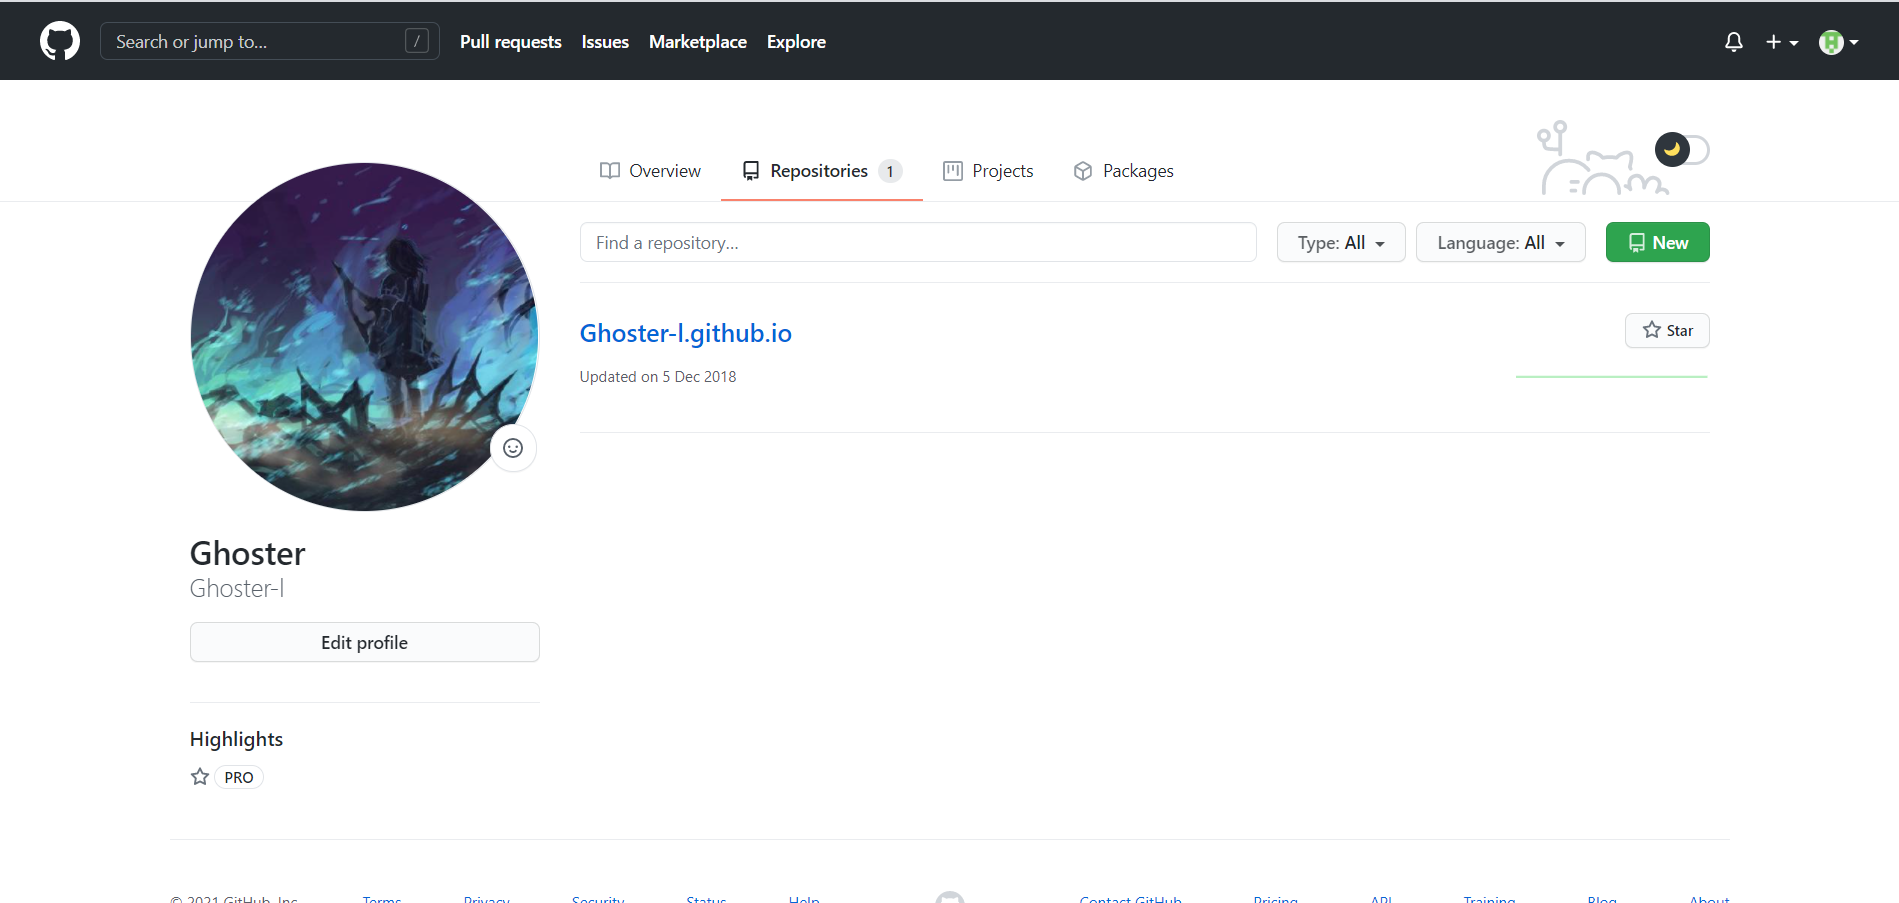
\includegraphics[scale=0.15]{github}
		\caption{Github}
		Github个人页:https://github.com/Ghoster-l
     \end{figure}
	    \begin{figure}[ht]
		\centering
		
\includegraphics[scale=0.15]{bilibili}
		\caption{bilibili}
	\end{figure}
    \begin{figure}[ht]
	\centering
	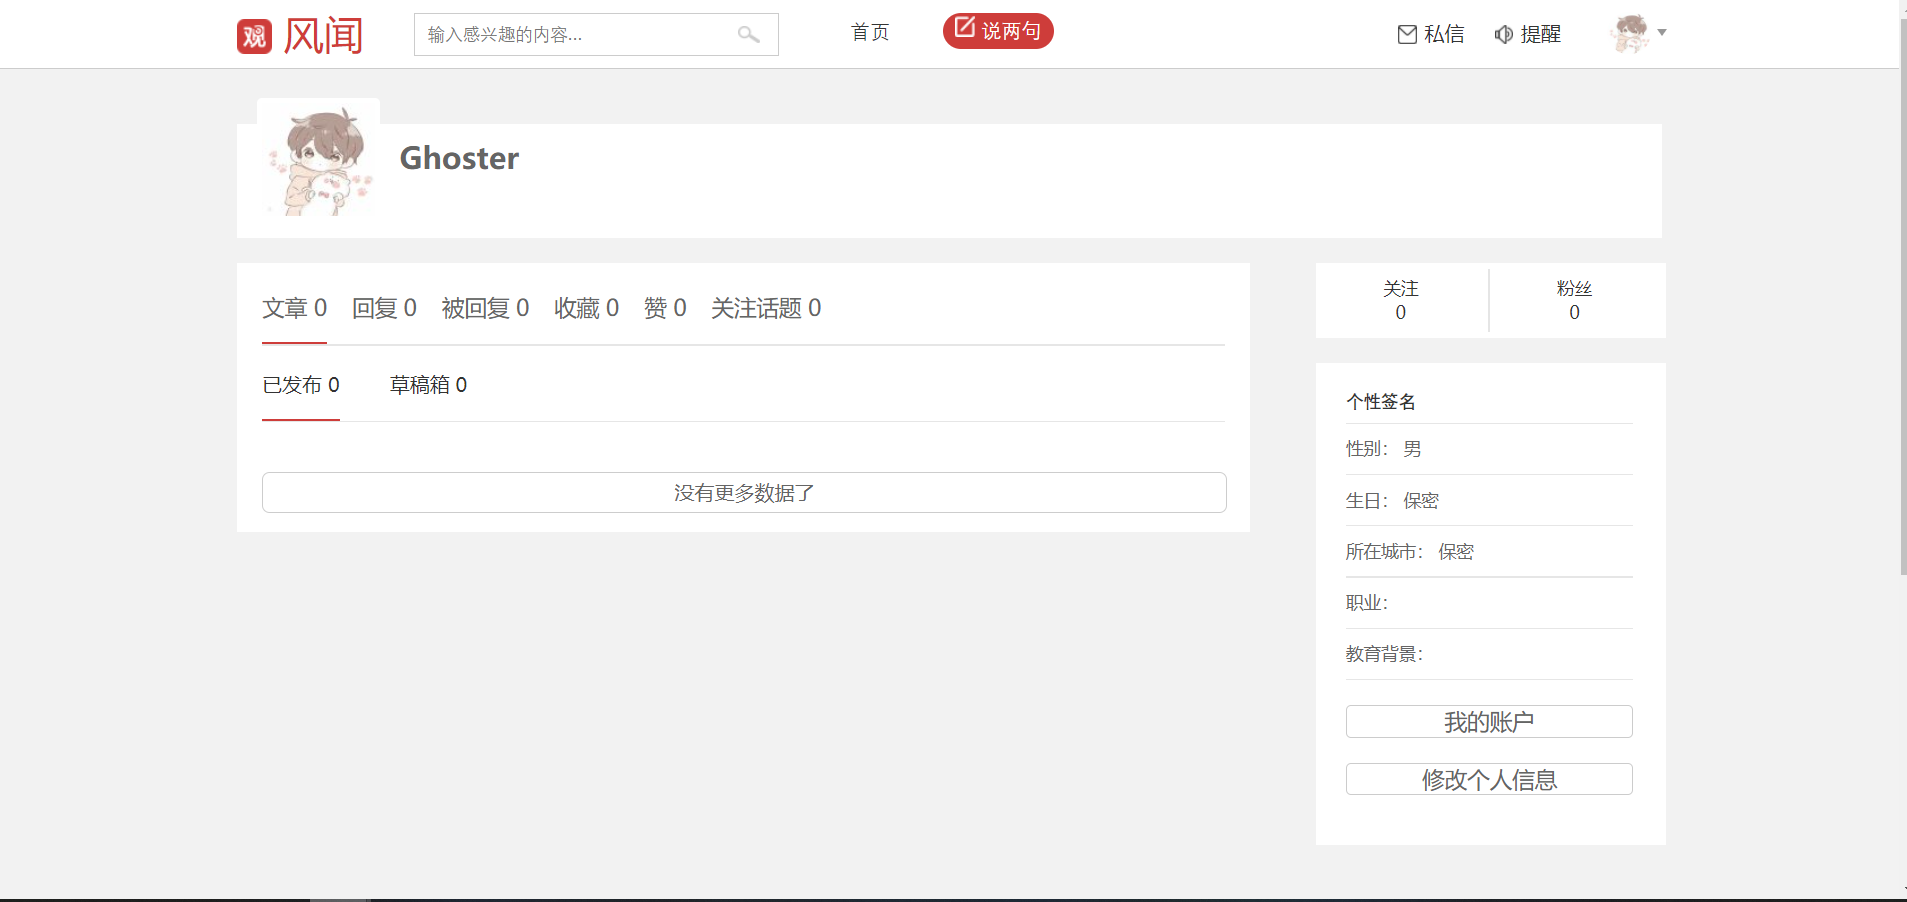
\includegraphics[scale=0.15]{guancha}
	\caption{观察者网}
	\end{figure}
	\begin{figure}[ht]
	\centering
	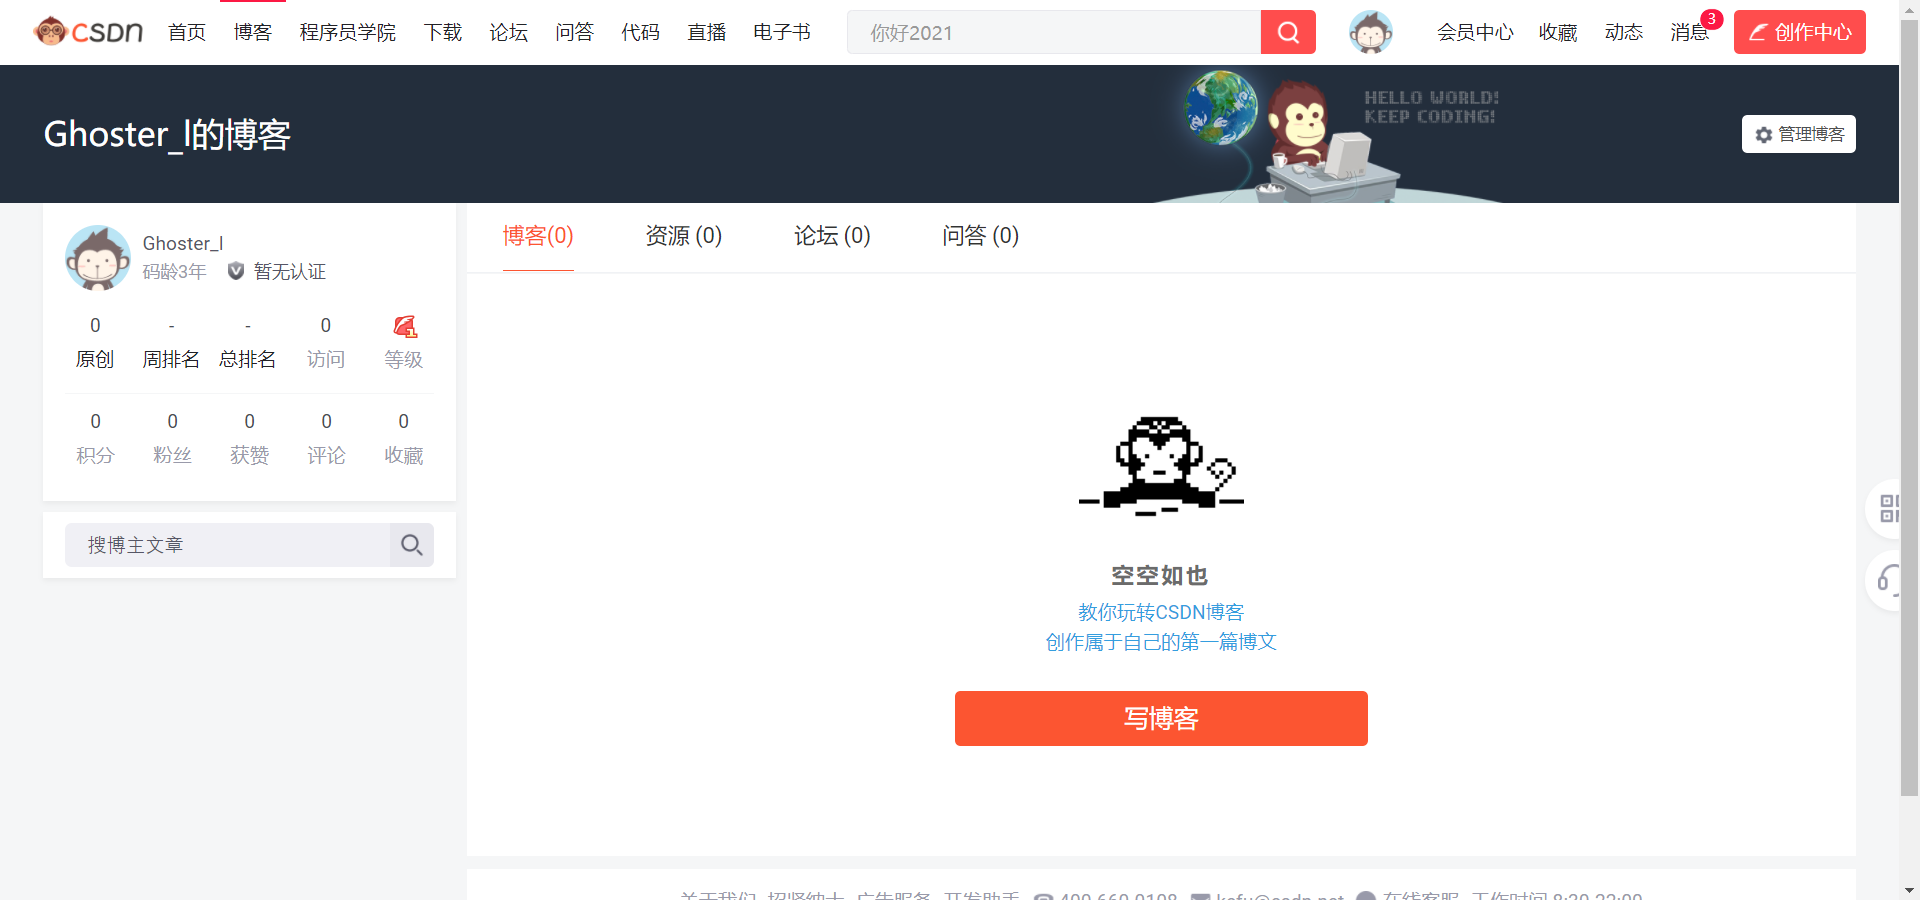
\includegraphics[scale=0.15]{csdn}
	\caption{csdn}
	\end{figure}
	\begin{figure}[ht]
		\centering
		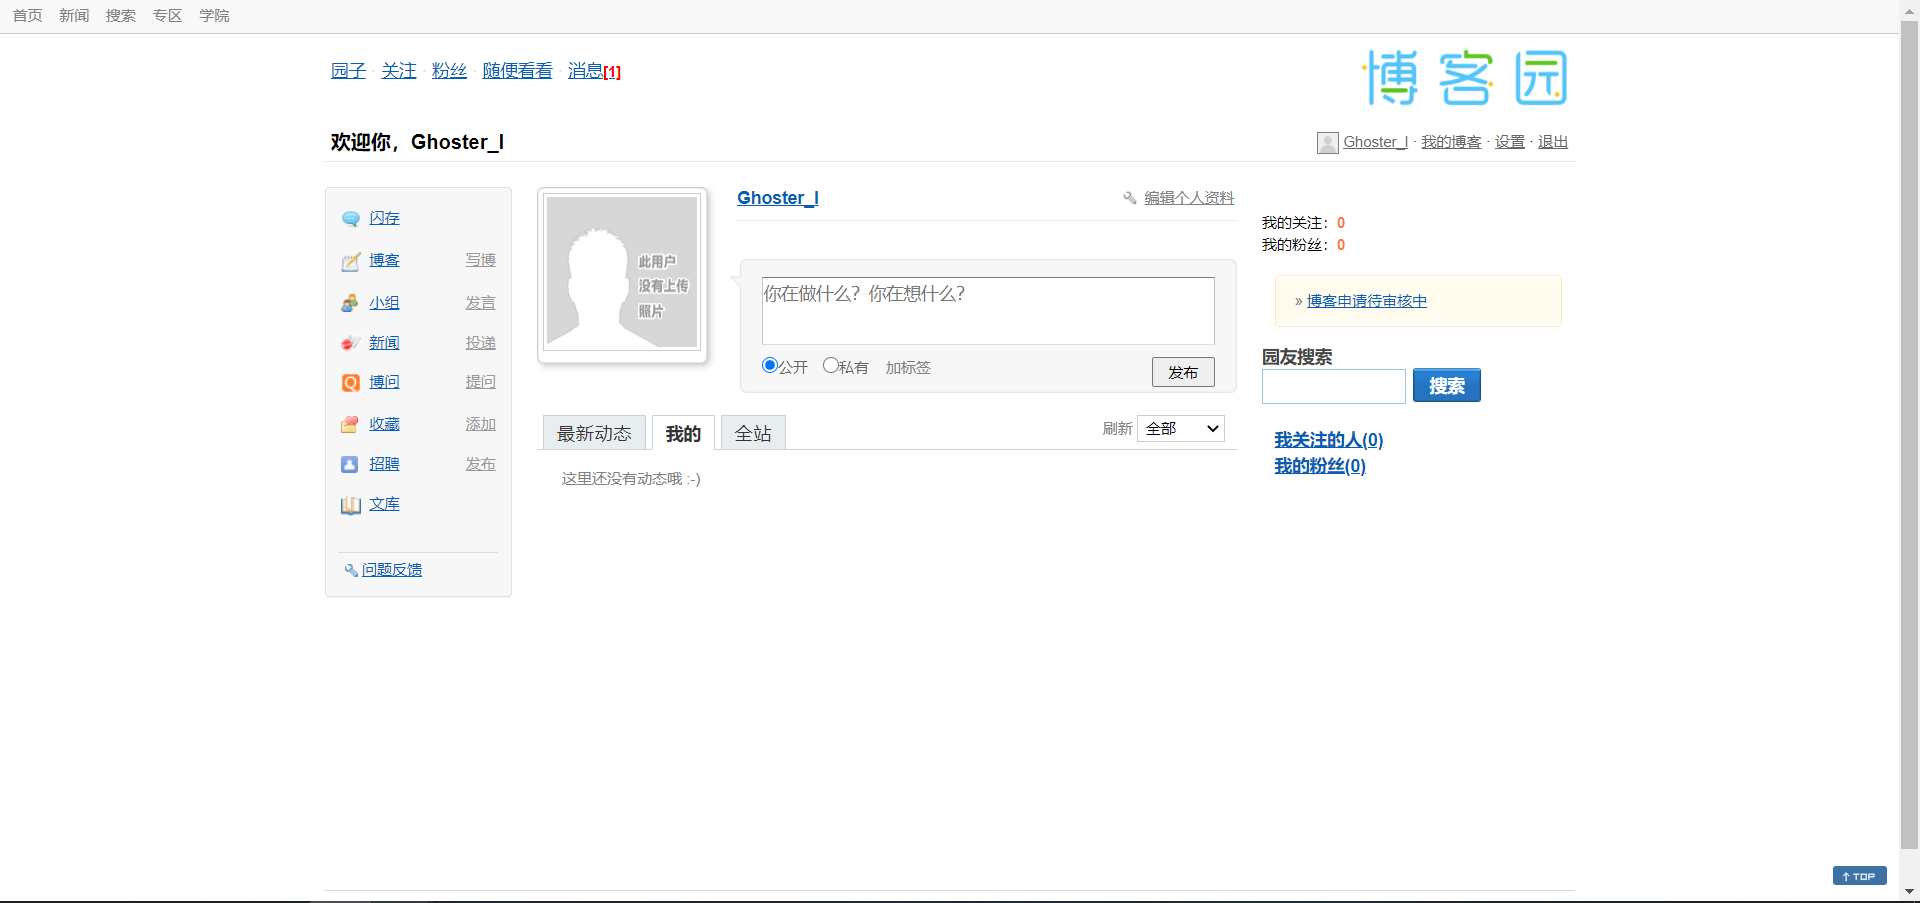
\includegraphics[scale=0.15]{boke}
		\caption{博客园}
	\end{figure}
	\begin{figure}[ht]
		\centering
		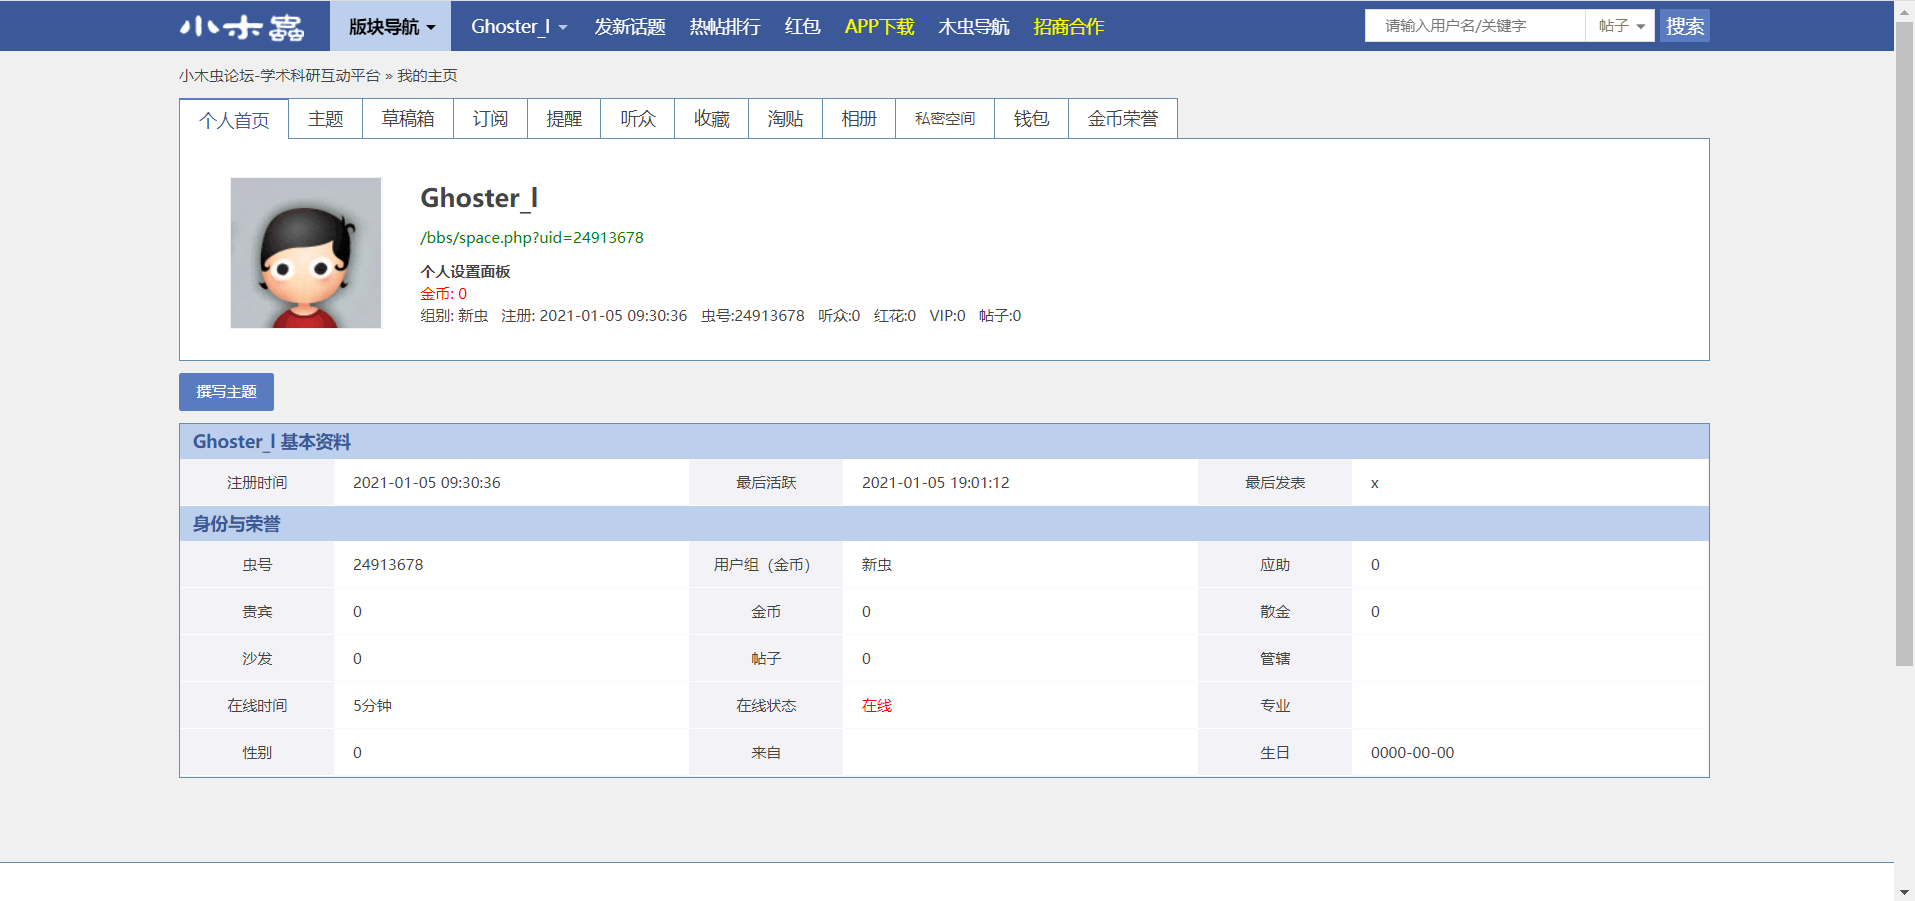
\includegraphics[scale=0.15]{xiaomuchong}
		\caption{小木虫}
	\end{figure}
\end{document}